\documentclass[11pt,a4paper]{article}
\usepackage[top=1.2cm, bottom=1.8cm, left=1.8cm, right=1.8cm]{geometry}

\usepackage[title]{appendix}
\usepackage{float}
\usepackage{subfig}
\usepackage[singlelinecheck=false]{caption}
\usepackage{graphicx}
\usepackage{listings}
\usepackage{color}
\usepackage[utf8]{inputenc}
\usepackage[english]{babel}
\usepackage{minted}

\usepackage[style=authoryear, backend=biber]{biblatex}
\addbibresource{main.bib}

\title{COMP6202: Assignment 2}
\author{
David Jones \\
dsj1n15@soton.ac.uk, ID: 27549836}
\date{}
\setlength{\intextsep}{1mm}

\begin{document}

\maketitle
% \begin{abstract}
%     This tidwd w
% \end{abstract}
\section{Introduction}
\textbf{Paper Re-Implemented:}\\
Coevolutionary Dynamics in a Minimal Substrate \parencite{Watson:2001}
\subsection{Experiments}
The experiments described by \cite{Watson:2001} are designed to demonstrate aspects of a co-evolutionary genetic algorithm (GA) implementation that can go wrong. This is handled using a simple and assessable \textit{substrate}. Specifically, a fixed length bitstring or fixed list of bitstrings.\\

\noindent the counting of ones in a 


to reduce bias bit flipping is not used.
fully assessable 
disengagement (loss of gradient)
2. over-specialization (Focussing)
3. relativism


Paper demonstrating:
* Intrinsitiviity
* 
* Relativitism
* Loss of gradient
If it fails on the simple example, more than likely to also occur for complex examples

The subjective fitness can be considred as the relative fitness, or an individauls actual knowledge of its fitness without knowledge of the objective metric

\subsection{Implementation}
Values are treated as a list of integers where each integer is considered a trait, this can
be considered as a specific skill. For simplicity 
Implemented with fitness proportionate selection. Modelled as a \textit{roulette wheel}. As the wheel will not `spin` when encountering individauls where $O_s^i=0$ a fixed bias that is close to 0 ($b = 1e-5$) is used.
The exact randomisation seeds to create the provided plots are in the source code; these are heavily dependentant on implementation and are likely only relevant for the source provided.

to ensure roulette wheel spins. This ensures the wheel \texttt{spins}, otherwise  first individual avoids guarenteed selection of the first individual in a population and

Although the original paper is n
It is not clear from the original papers which properties to use 
The individual properties were not specified explicity in the original paper, h $T_l=50$ and $T_n=2$

% Introduction: You need not spend more than 1.5 pages describing the original paper.
% o briefly describe the paper/experiment
% o What you evolved including
% o How you represented individuals
% o What fitness function did you define
% o What kind of GA you used
% o Steady state/ generational? Tournament selection/ fitness proportionate (roulette
% wheel)?
% o What kind of crossover (if any) you used.
% o All parameters (enough detail so a reader could re-implement the GA)


\section{Reimplementation Results}
Figure \ref{fig:figure_5} highlights a disconnnect between the objective score and subjective scoring method.
One of the downsides of this selection method is that if populations start to disengage, the population will be rapidly replaced with the same individual. This reduces diversity.
The requirements to re-engage are very small. 1/15 
\begin{figure}[H]
    \centering
    \begin{tabular}{cc}
    \subfloat[Original \parencite{Watson:2001}]{\includegraphics[height=6.5cm]{original/fig3.png}}
    \hspace{1.5mm}
    \subfloat[Reimplementation]{\includegraphics[height=6.5cm]{plots/fig3.pdf}}
    \end{tabular}
    \caption{$I=(1, 100), S=1$ \textit{(Originally Figure 3)}}
    \label{fig:figure_3}
\end{figure}

\begin{figure}[H]
    \centering
    \begin{tabular}{cc}
    \subfloat[Original \parencite{Watson:2001}]{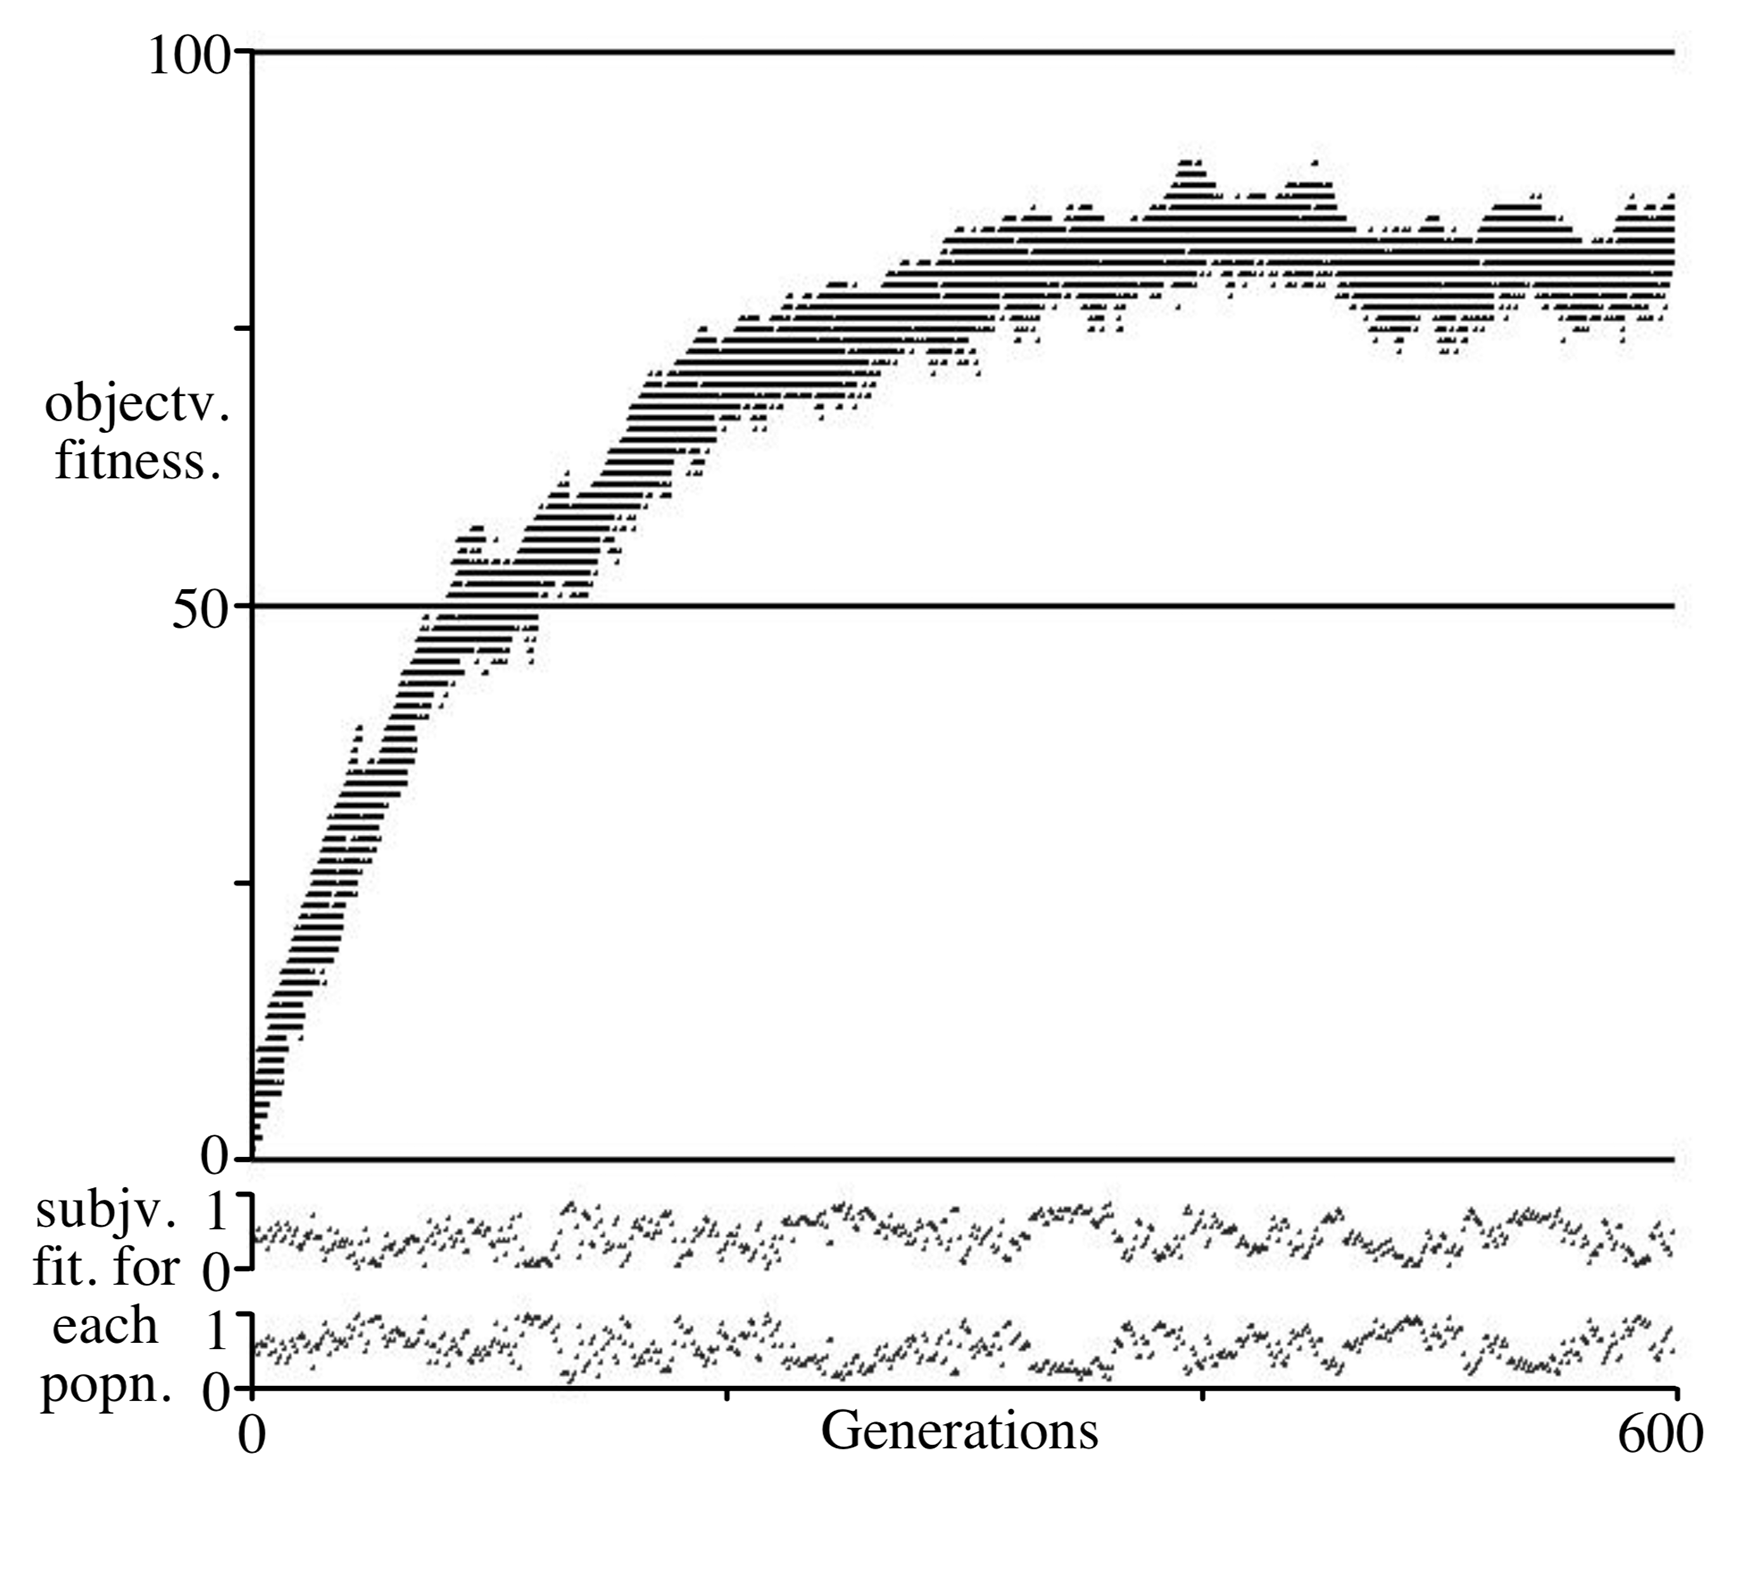
\includegraphics[height=6.5cm]{original/fig4.png}}
    \hspace{1.5mm}
    \subfloat[Reimplementation]{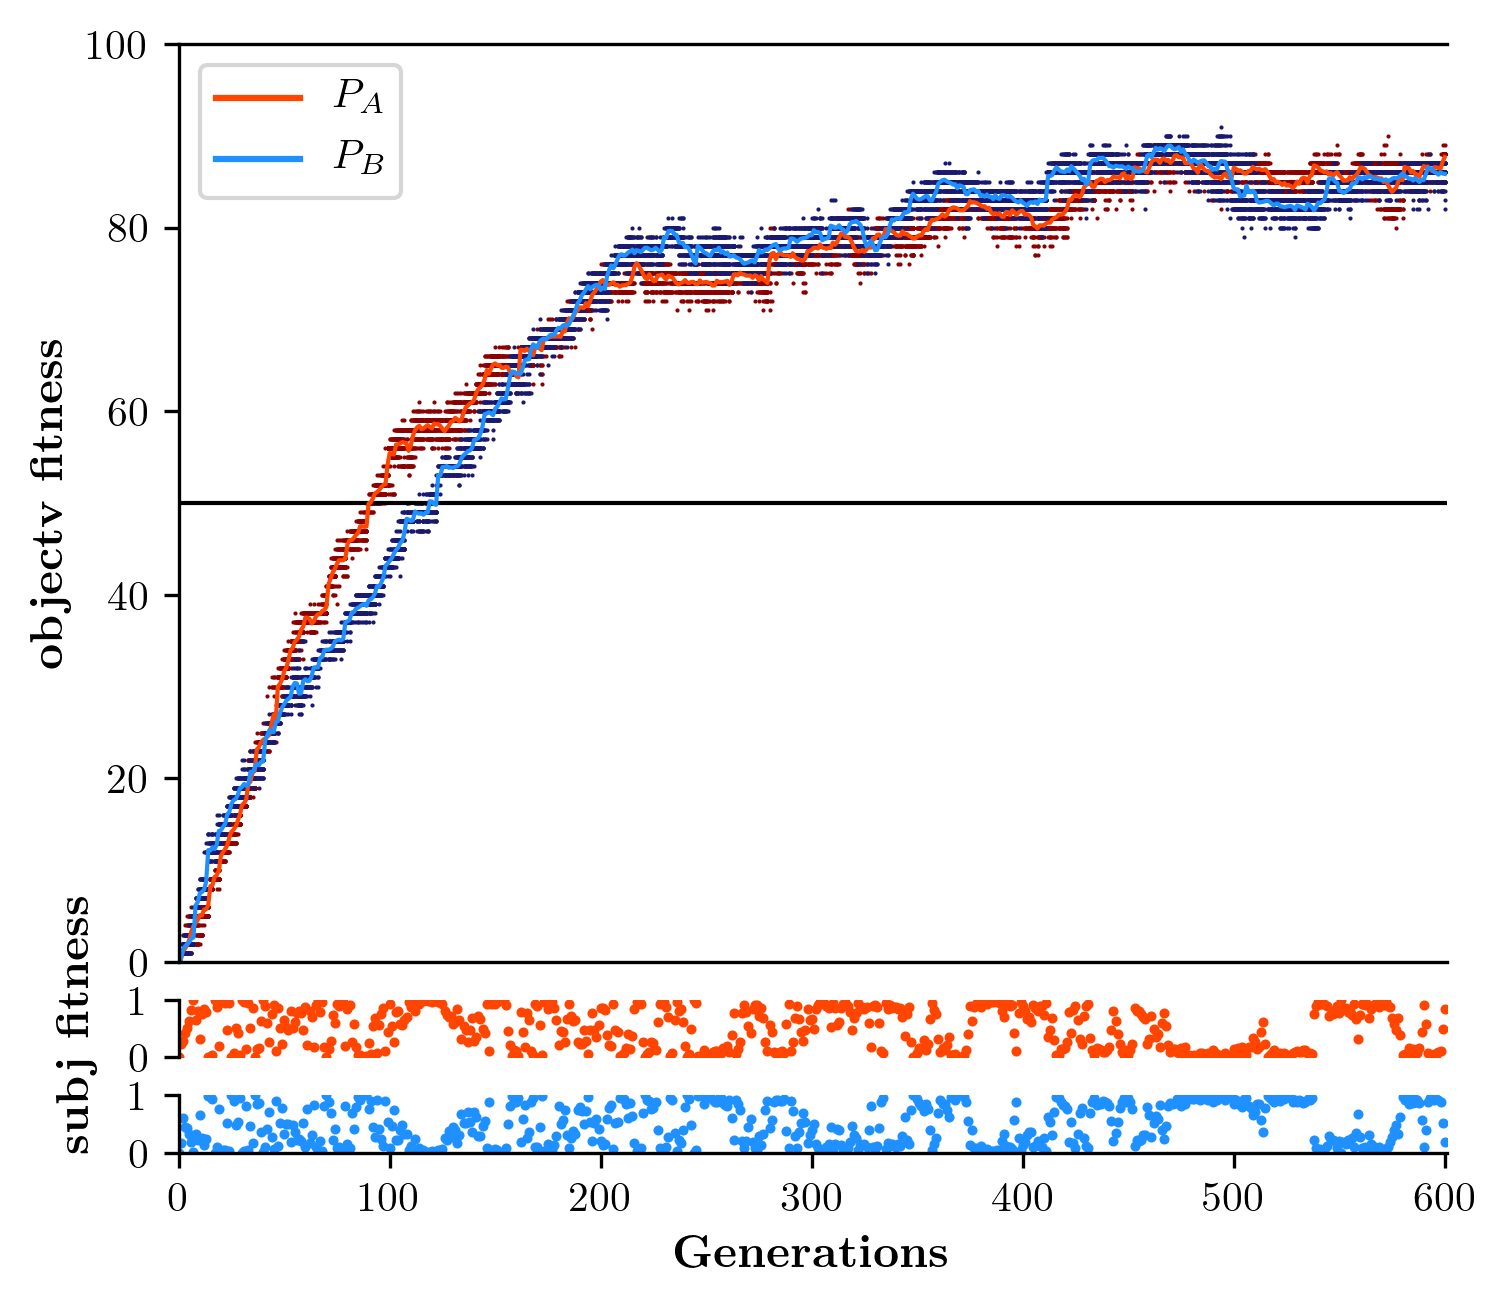
\includegraphics[height=6.5cm]{plots/fig4.pdf}}
    \end{tabular}
    \caption[]{$I=(10, 10)$ \textit{(Originally Figure 4)} }
    \label{fig:figure_4}
\end{figure}

\begin{figure}[H]
    \centering
    \begin{tabular}{cc}
    \subfloat[Original \parencite{Watson:2001}]{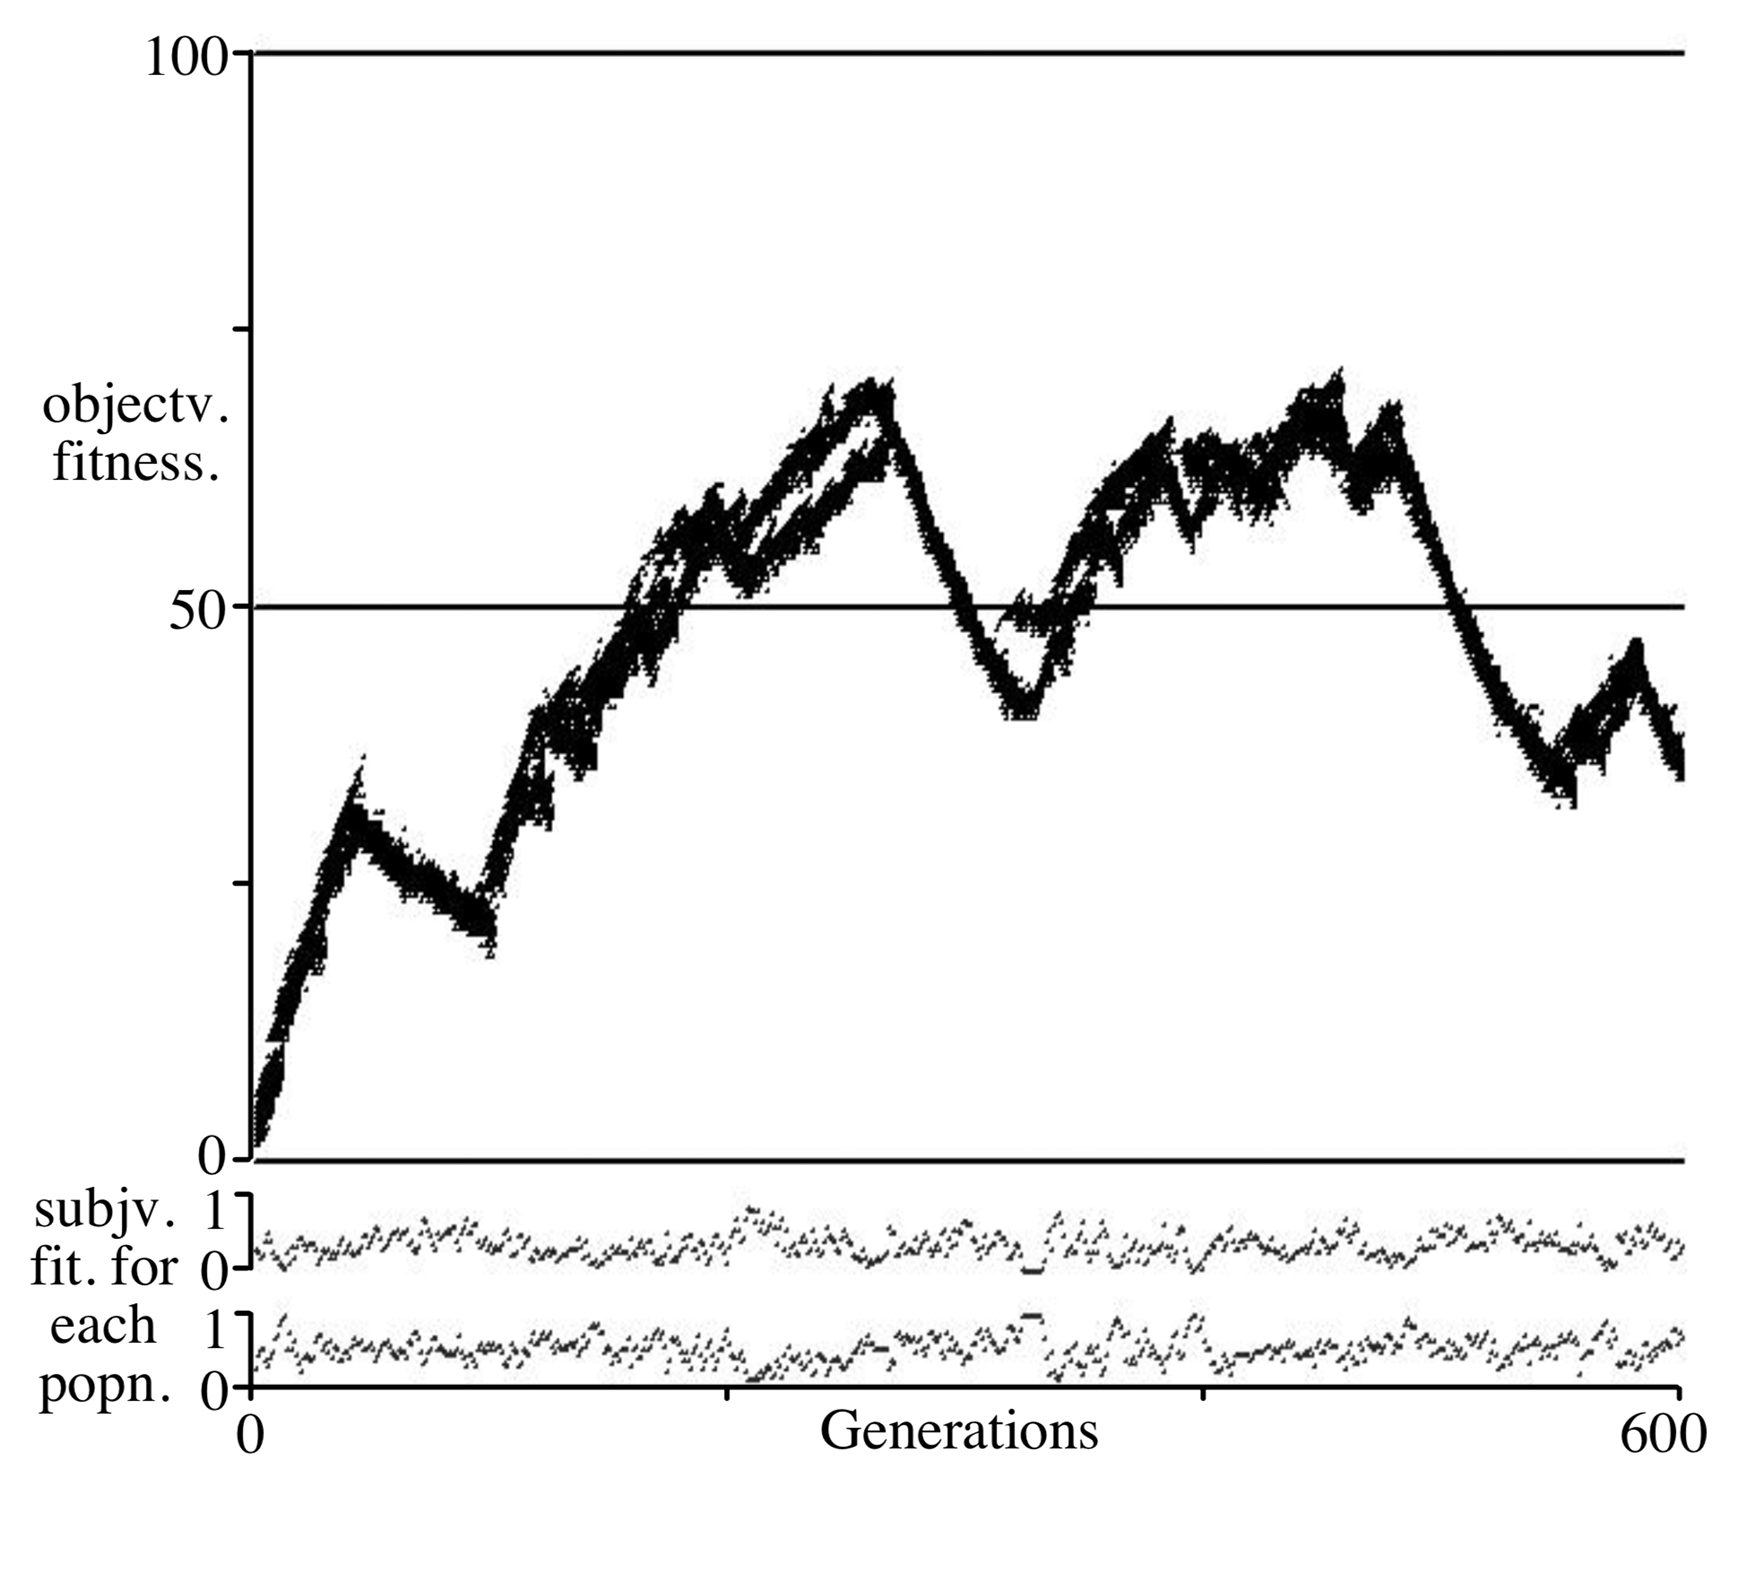
\includegraphics[height=6.5cm]{original/fig5.png}}
    \hspace{1.5mm}
    \subfloat[Reimplementation]{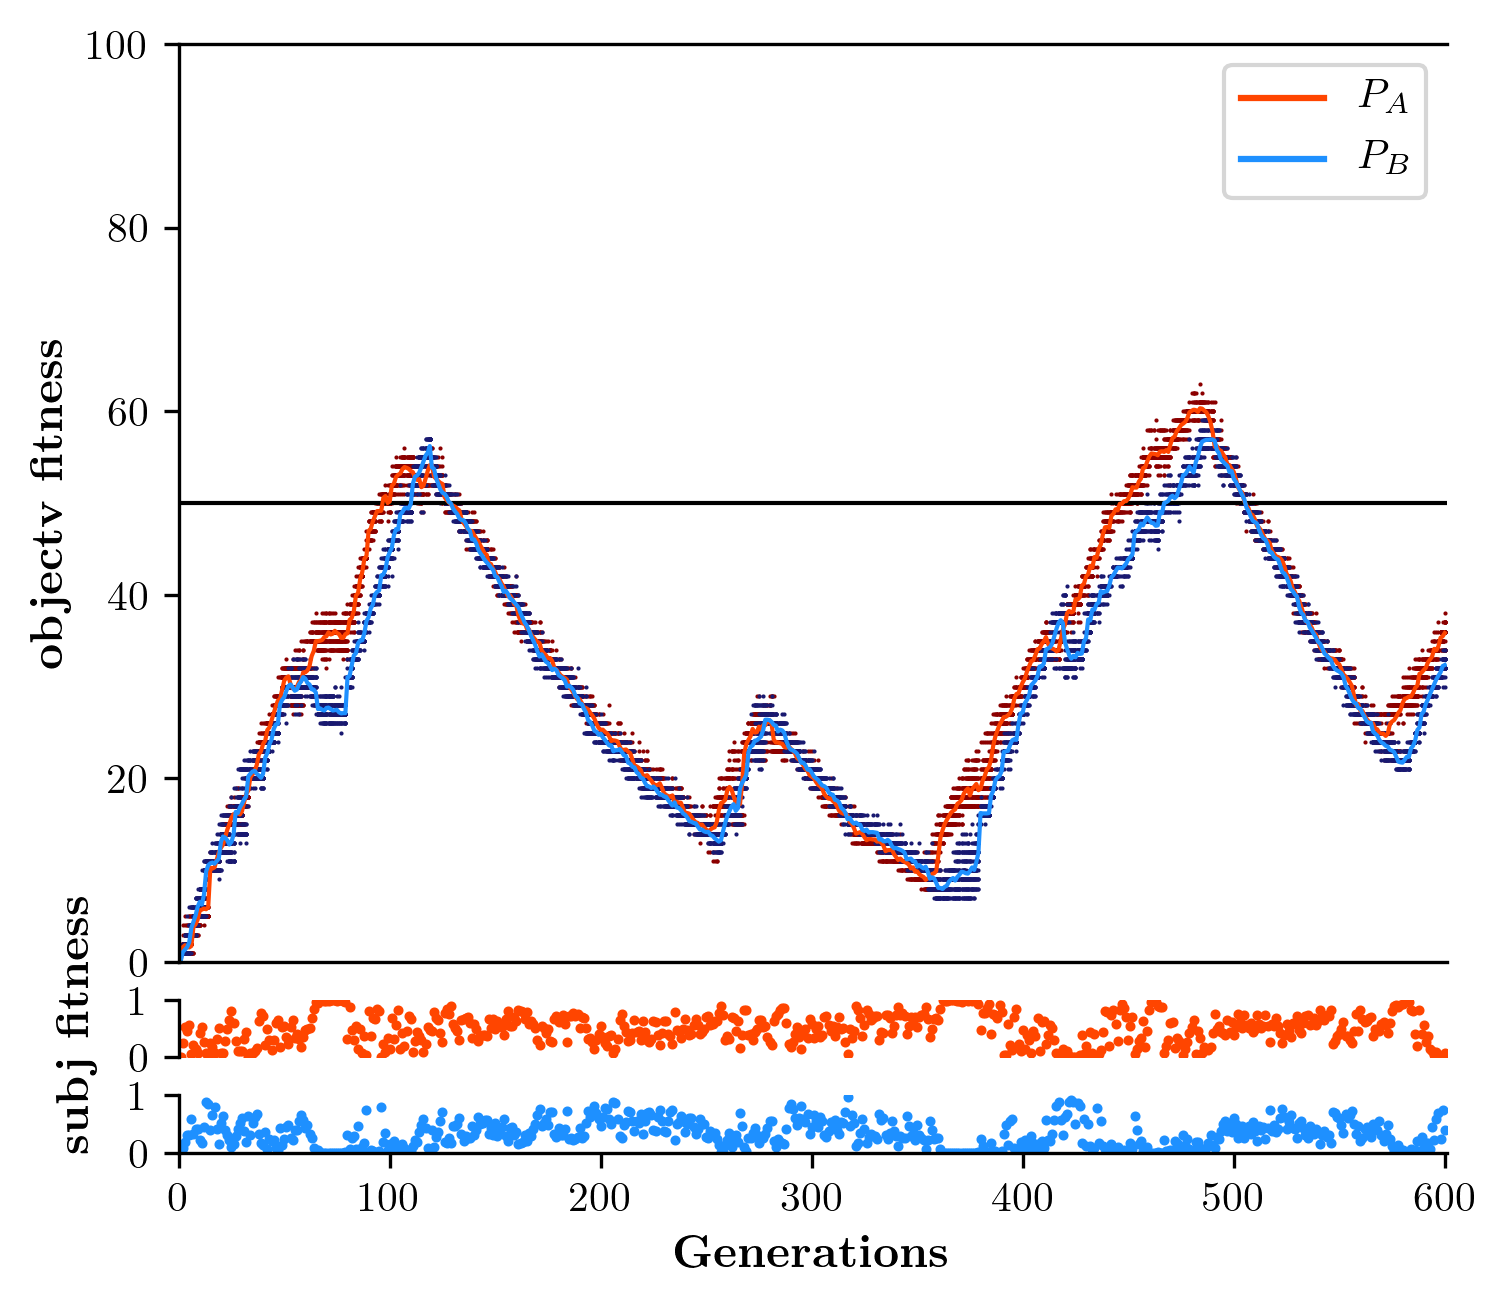
\includegraphics[height=6.5cm]{plots/fig5.pdf}}
    \end{tabular}
    \caption[]{$I=(10, 10)$, Intransitive \textit{(Originally Figure 5)}}
    \label{fig:figure_5}
\end{figure}
No iterations went over obj fit of 50.
Can see driven down nature beyond reasonable drift. Not always happening at polarisation points. more polarisation than excepcted across full range.

\section{Extension}
\subsection{Hypothesis}
\subsection{Implementation}
\subsection{Results}
\section{Conclusion}

\printbibliography

\begin{appendices}
\section{Extra Figures}
\begin{figure}[H]
    \centering
    \begin{tabular}{cc}
    \subfloat[Original \parencite{Watson:2001}]{\includegraphics[height=6.5cm]{original/fig1.png}}
    \hspace{1.5mm}
    \subfloat[Reimplementation]{\includegraphics[height=6.5cm]{plots/fig1.pdf}}
    \end{tabular}
    \caption{$S=15$ \textit{(Originally Figure 1)}}
    \label{fig:figure_1}
\end{figure}
\begin{figure}[H]
    \centering
    \begin{tabular}{cc}
    \subfloat[Original \parencite{Watson:2001}]{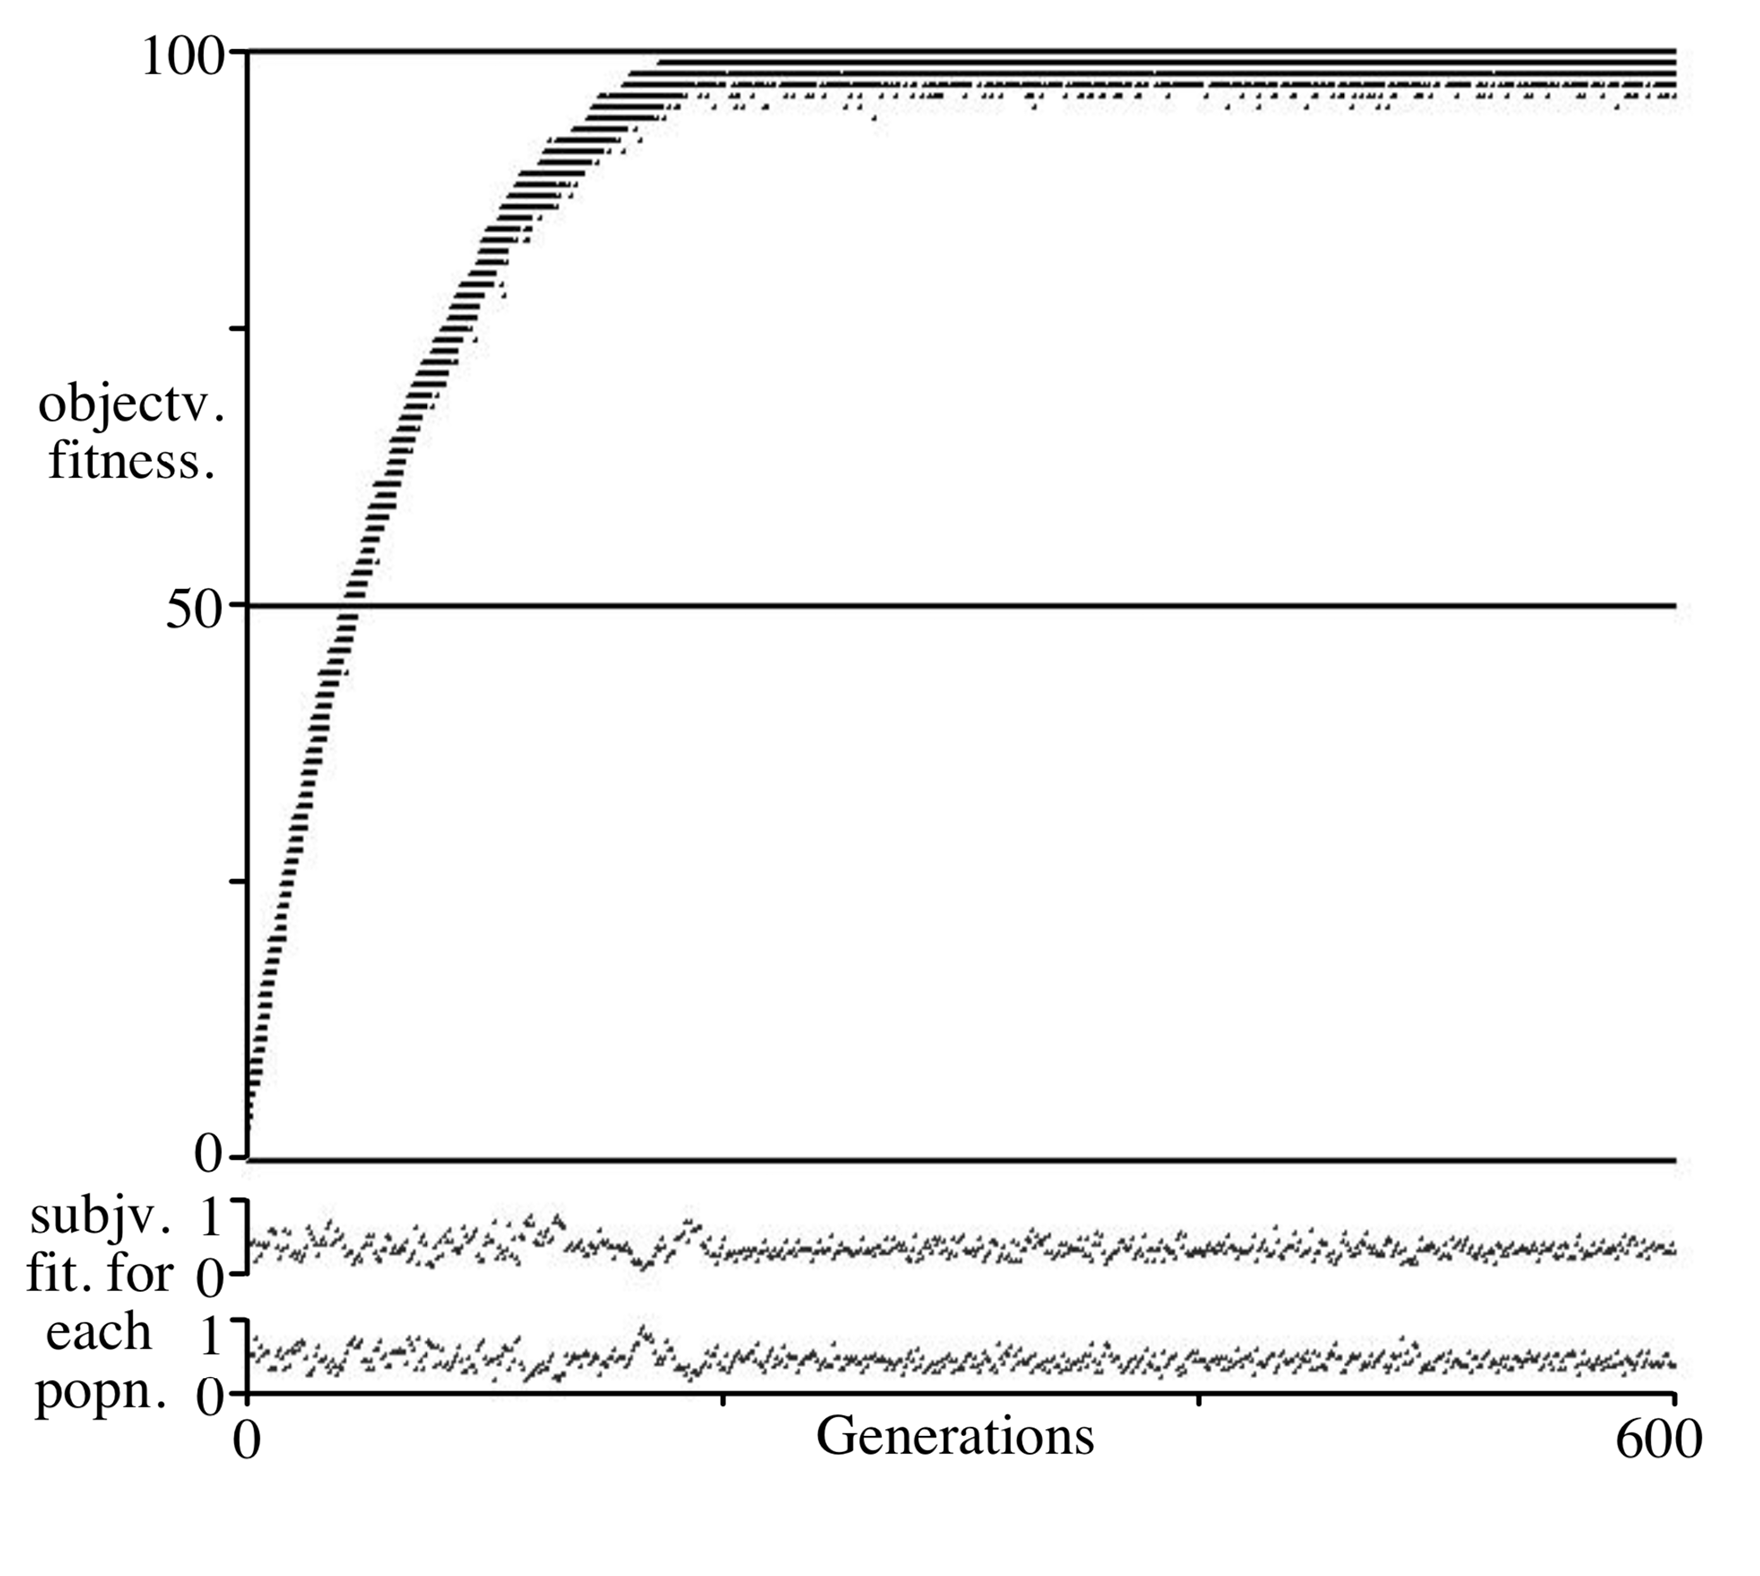
\includegraphics[height=6.5cm]{original/fig2.png}}
    \hspace{1.5mm}
    \subfloat[Reimplementation]{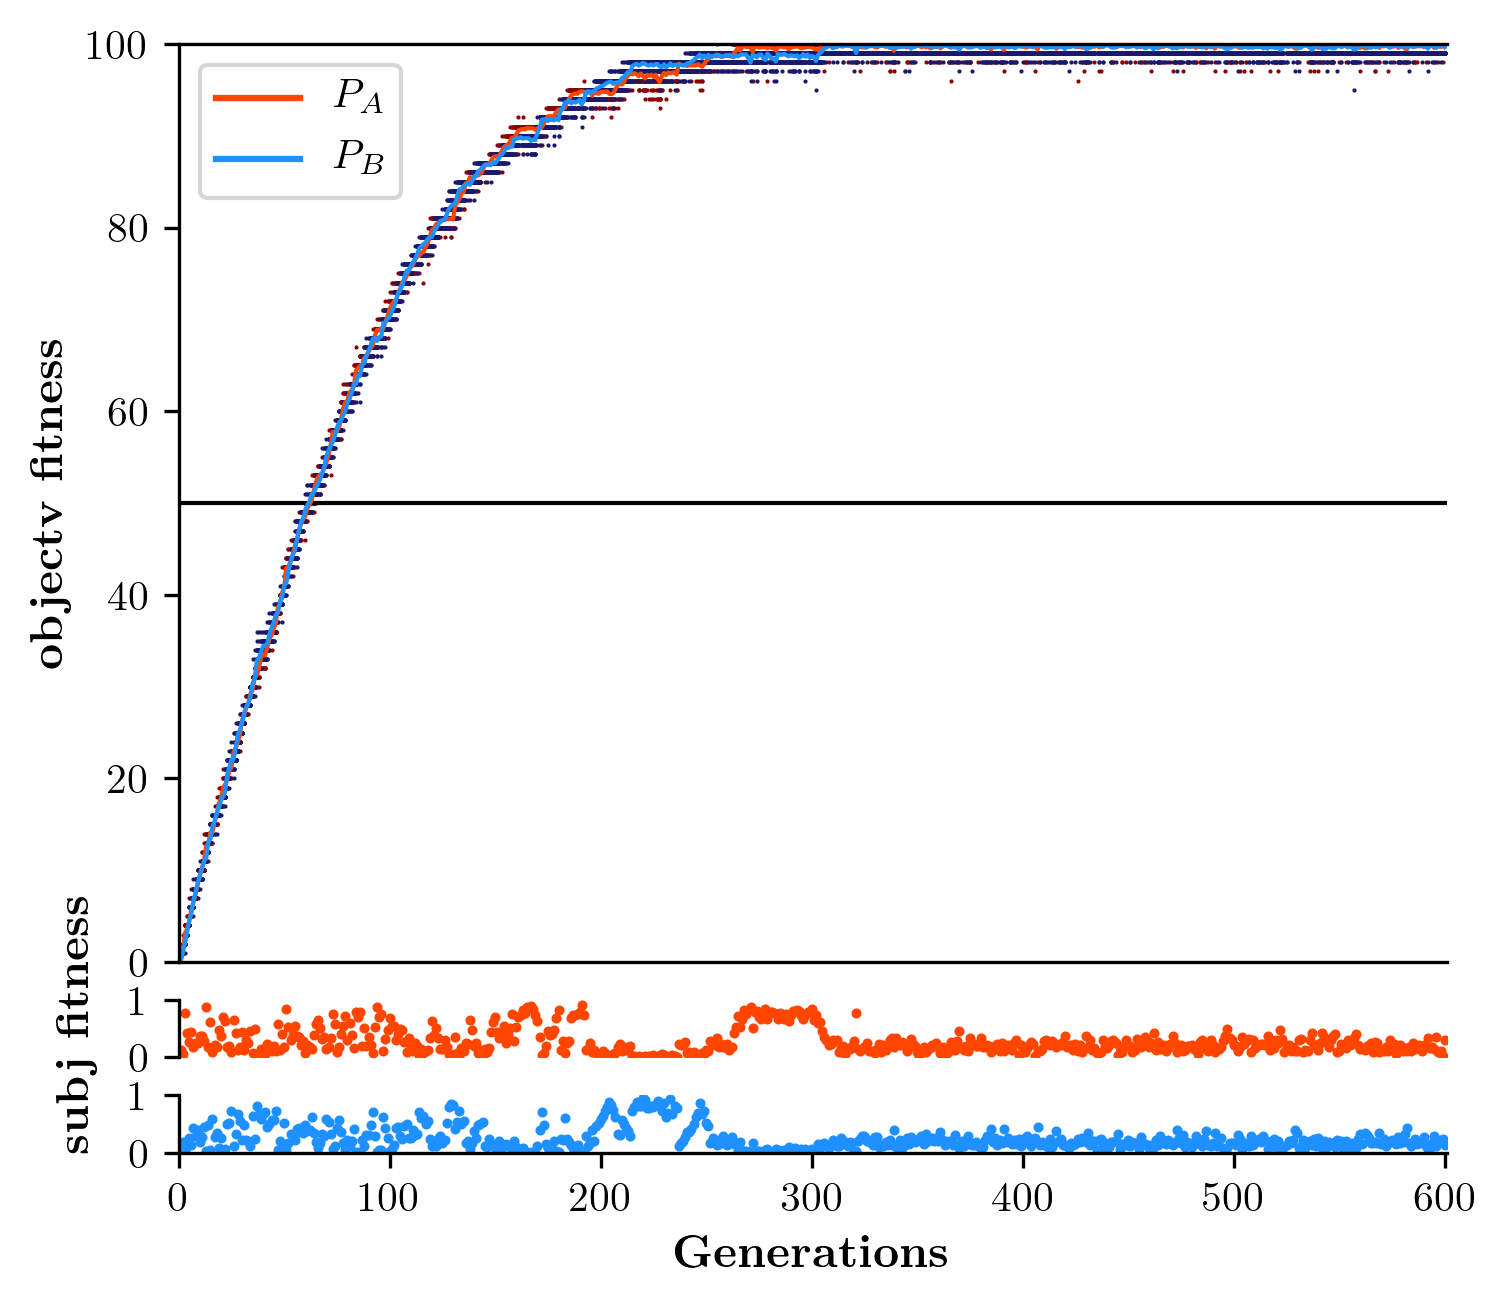
\includegraphics[height=6.5cm]{plots/fig2.pdf}}
    \end{tabular}
    \caption{$S=15$ \textit{(Originally Figure 2)}}
    \label{fig:figure_2}
\end{figure}

\newpage
\section{Code Listings}
\subsection{assignment2.py}
\inputminted{python}{../code/assignment2.py}\newpage
\subsection{coevolution.py}
\inputminted{python}{../code/coevolution.py}\newpage
\subsection{representation.py}
\inputminted{python}{../code/representation.py}\newpage
\subsection{mutation.py}
\inputminted{python}{../code/mutation.py}\newpage
\subsection{scoring.py}
\inputminted{python}{../code/scoring.py}\newpage
\subsection{selection.py}
\inputminted{python}{../code/selection.py}\newpage
\subsection{plot.py}
\inputminted{python}{../code/plot.py}\newpage
\subsection{utils.py}
\inputminted{python}{../code/utils.py}\newpage


\end{appendices}



\end{document}